\section{LEP and the OPAL detector}
\subsection{LEP}
%LEP luftaufnahme
\begin{figure}[ht]
	\centering
	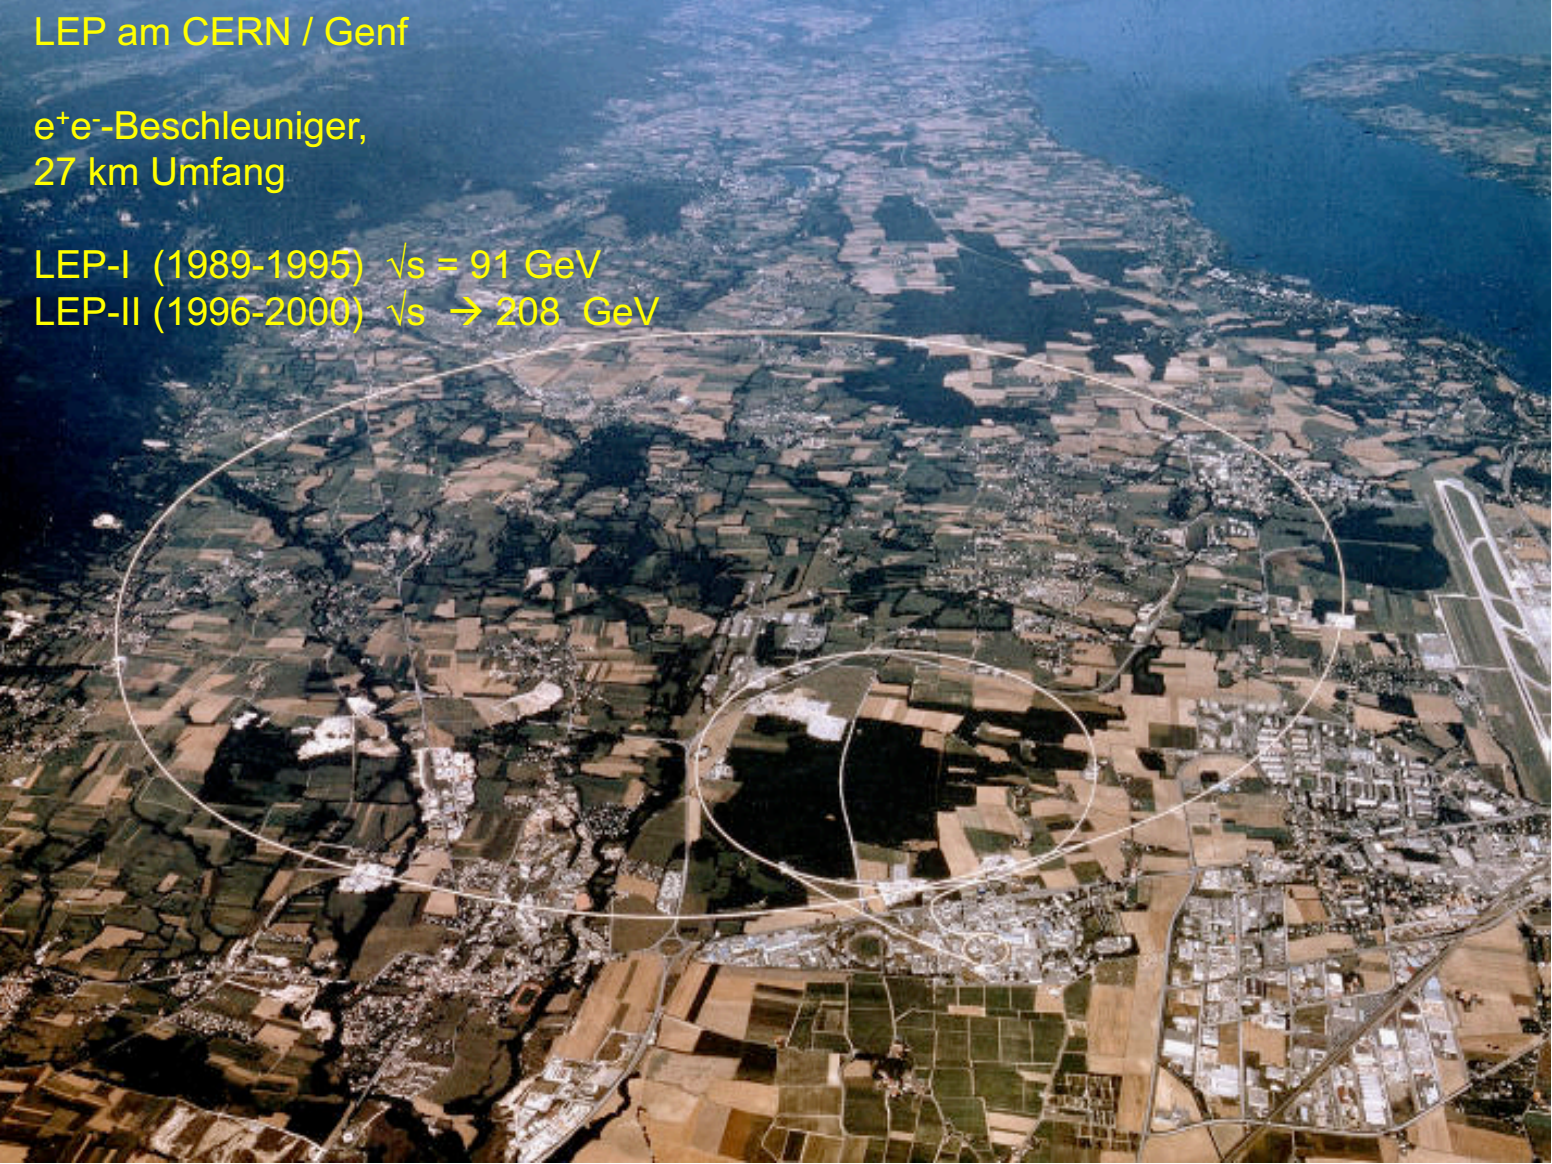
\includegraphics[width=1.0\linewidth]{graphics/LEPmap}
	\caption[Bird's eye view LEP]{Bird's eye view of the Large Electron-Positron Collider at Cern in Geneva, Switzerland. Today the large circular collider tunnel is used for the Large Hadron Collider (LHC)\cite{jakobs}. The smaller circle belonged to the Super Proton Synchroton (SPS) experiment.}
	\label{fig:LEPmap}
\end{figure}
The Large Electron-Positron Collider is storage ring with a diameter of 27 km. It accelerated 4 bunches of $4\cdot 10^{11}$ electrons and positrons in opposite directions for about 20 hours. At four predetermined points (the positions of the detectors: Aleph, Delphi, L3 and OPAL) the beams collided about every 25$\mu s$, but the reaction $e^+ e^- \rightarrow f \bar{f}$ only occurred at a frequency of roughly 1Hz\cite{muenchen}.

\subsection{OPAL}
The OPAL detector consists of several, in shells arranged, components(s.figure \ref{fig:OPALaufbau}). Closest to the beam is the central tracking chamber (red), enabling tracking of charged particles. It is followed by the electromagnetic calorimeter (cyan ), which is used to determine the energy of positrons, electrons and photons.
Then comes the hadronic calorimeter (yellow) measuring the energy of hadrons passing through the electromagnetic calorimeter.
The outermost shell are the muon detectors(blue), as name suggests used to detect muons\cite{cern}.\\

%schematischer OPAL-Aufbau
\begin{figure}[ht]
\centering
\includegraphics[width=1.0\linewidth]{graphics/OPALaufbau}
\caption[[Opal schematic build up]]{The OPAL detector's schematic build up}
\label{fig:OPALaufbau}
\end{figure}

\paragraph{Tracking chamber}
The Tracking chamber is a multi-wire chamber: Anode wires are spanned between two cathode plates. Each of those wires can be read out separately. At constant drift velocity, the 
%elektromagnetisches Kaloriemeter
\begin{figure}[h]
\centering
\includegraphics[width=1.0\linewidth]{"graphics/elektromagnetisches kaloriemeter"}
\caption[electromagnetic calorimeter]{construction of the electromagnetic calorimeter}
\label{fig:elektromagnetischeskaloriemeter}
\end{figure}
